% class
\documentclass[a4paper,12pt,xelatex,ja=standard]{bxjsarticle}

% packages
%% mathematical notations
\usepackage{amsthm,amsmath,amssymb,amsfonts} % mathematical notations
\usepackage{bm} % bold character
\usepackage{latexsym} % more mathematical notations
\usepackage{physics} % physical notations
\usepackage{mathtools} % math tools
%% graphs
\usepackage{graphicx, xcolor} % graph
\usepackage{circuitikz} % for circuit elements
\usepackage{float} % positioning of graphs
\usepackage{siunitx} % SI units
\usepackage{tikz} % graphic elements
\usepackage{wrapfig} % must be after float package.
\usepackage{askmaps} % Karnaugh map
%% type system
\usepackage{bussproofs} % proof tree
%% code
\usepackage[ruled,vlined]{algorithm2e} % pseudo code
\usepackage{listings} % source code
\usepackage{inconsolata}
\lstset{
  basicstyle=\footnotesize,
  numbers=left,
  frame={tb}
}
\usetikzlibrary{automata, positioning, calc, quotes}
\tikzset{
  ->,
  >={Stealth[round]},
  auto,
  every state/.style={draw},
  node distance=3cm
}
\newcommand\DoubleLine[5][4pt]{%
    \path(#2)--(#3)coordinate[at start](h1)coordinate[at end](h2);
    \draw[<-,very thick,black] ($(h1)!#1!90:(h2)$)  to ["#4"]   ($(h2)!#1!-90:(h1)$);
    \draw[->,very thick,  red] ($(h1)!#1!-90:(h2)$) to ["#5" '] ($(h2)!#1!90:(h1)$);
    }

% Basic information
\title{電子情報学専攻 \, 専門 \\ 令和2年 \, 解答・解説}
\author{diohabara}
\date{\today}

\begin{document}
\maketitle

\section*{第1問\ 電気・電子回路}

\section*{第2問\ 論理回路}
\subsection*{(1)}
状態を持つ論理回路。入力と状態から、出力と次の状態が決まる。

\subsection*{(2)}
TODO
% $X_k \times 2^{i-k}$を6で割ったあまりで考えると$k=i$のとき1で、それ以降は2と4が連続する。よって$i$から考えていくと以下のようなミーリーグラフとなる。

% \begin{figure}[H]
%   \centering
%   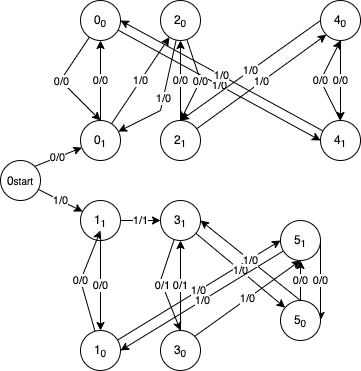
\includegraphics[height=5cm]{images/2021_2_automaton.png}
% \end{figure}

\subsection*{(3)}
\subsection*{(4)}
\subsection*{(5)}
\subsection*{(6)}

\section*{第3問\ アルゴリズムとデータ構造}
\subsection*{(1)}
\subsection*{(2)}
\subsection*{(3)}
\subsection*{(4)}
\subsection*{(5)}

\section*{第4問\ ネットワーク}

\section*{第5問\ 信号処理}
\subsection*{(1)}
\subsection*{(2)}
\subsection*{(3)}
\subsection*{(4)}
\subsection*{(5)}
\subsection*{(6)}
\subsection*{(7)}

\end{document}
